% Lydia Lee, lydia.lee@berkeley.edu
\qns{Automatic Gain Control}

\begin{enumerate}
\qitem\label{amp}{
	Design a circuit where $V_\text{out} = -10V_\text{in}$. You are allowed to use
	\begin{itemize}
		\item op amps: $\leq$1. You do not need to specify rail voltages for this subpart.
		\item resistors: as many as you want
		\item capacitors: as many as you want
	\end{itemize}
}
\empt{
	\vspace{1.5cm}
	\begin{circuitikz}
		\draw
		(0,0) to[short] ++(-1,0)
			to[sV,v_=$V_\text{in}$] ++(0,-2)
			node[ground] () {};
	\end{circuitikz}
	\vspace{1.5cm}}

\qitem\label{no_rail}{
	Your design was provided voltage rails at $5\si{\volt}$ and $-5\si{\volt}$, and that your input signal looks like so:
	\begin{center}
		\begin{tikzpicture}[scale=0.75, transform shape]
\begin{axis}[
    axis lines = middle,
    ylabel = {$V_\text{in}(t)$},
    xtick={0,1.57,3.14,4.71,6.28, 7.85, 9.42, 11.00, 12.57},
    xticklabels={$0$, $\frac{\pi}{2}$,$\pi\,$,$\,\,\,\frac{3}{2}\pi$,$\,\,\,2\pi$, $\frac{5}{2}\pi$, $3\pi$, $\frac{7}{2}\pi$, $4\pi$},
    ytick={0,-0.5,0.5,-1,1},
    ymin=-1.5,
    ymax=1.5,
    xmin = 0,
    xmax=4*pi
]
\addplot [
	color=black,
	domain=0:4*pi,
	samples=200
	]
	{ 0.5*sin(deg(x))
	};
\end{axis}
\end{tikzpicture}
	\end{center}
	Will your signal be faithfully amplified? That is, will your op amp distort the output because of railing/clipping?
}
\empt{\vspace{2cm}}

\qitem\label{yes_rail}{
	Again, your design has voltage rails at $\pm 5\si{\volt}$. Your input signal now looks like so:
	\begin{center}
		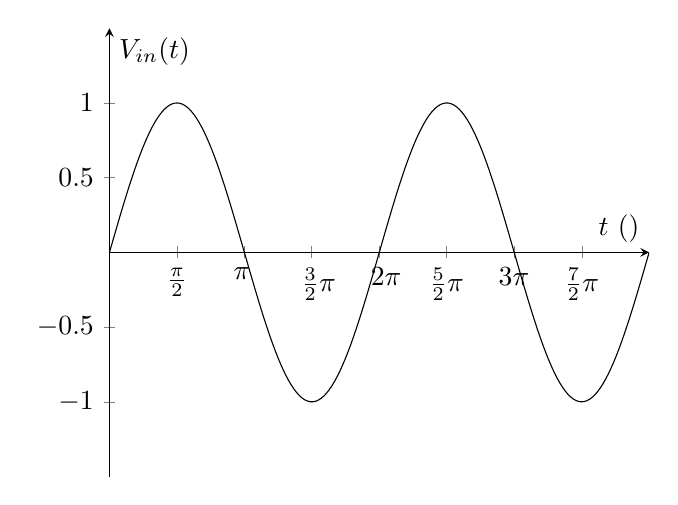
\begin{tikzpicture}
\begin{axis}[
    axis lines = middle,
    xlabel = {$t$ $(\si{\milli\second})$},
    ylabel = {$V_\text{in}(t)$},
    xtick={0,1.57,3.14,4.71,6.28, 7.85, 9.42, 11.00, 12.57},
    xticklabels={$0$, $\frac{\pi}{2}$,$\pi\,$,$\,\,\,\frac{3}{2}\pi$,$\,\,\,2\pi$, $\frac{5}{2}\pi$, $3\pi$, $\frac{7}{2}\pi$, $4\pi$},
    ytick={0,-0.5,0.5,-1,1},
    ymin=-1.5,
    ymax=1.5,
    xmin = 0,
    xmax=4*pi
]
\addplot [
	color=black,
	domain=0:4*pi,
	samples=200
	]
	{ sin(deg(x))  
	};
\end{axis}
\end{tikzpicture}
	\end{center}
	With this input signal, will your amplifier distort the output due to railing/clipping?
}
\empt{\vspace{2cm}}

\qitem\label{resistorDAC}{
	Design a circuit which can have a resistance $R$ when an input signal $\phi$ is low and a resistance $nR$ ($n > 1$) when $\phi$ is high. You may use:
	\begin{itemize}
		\item ideal switches: as many as you want
		\item resistors: $\leq 2$
	\end{itemize}
}
\empt{\vspace{4cm}}

\qitem\label{vga}{
	Using your answer from parts \ref{amp} and \ref{resistorDAC}, design a circuit where
	$$V_\text{out} = \begin{cases}
						-5V_\text{in} & \phi = 0\\
						-10V_\text{in} & \phi = V_{DD}
					\end{cases}$$
}
\empt{
	\vspace{2cm}

	\begin{circuitikz}
		\draw
		(0,0) to[short] ++(-1,0)
			to[sV,v_=$V_\text{in}$] ++(0,-2)
			node[ground] () {};
	\end{circuitikz}
	\vspace{2cm}}

\qitem\label{agc}{
	Now let's put it all together. Using
	\begin{itemize}
		\item op amps: as many as you want
		\item switches: as many as you want
		\item resistors: as many as you want
		\item ideal voltage source: as many as you want, not including the provided rails $\pm 5\si{\volt}$
	\end{itemize}
	design a circuit which adjusts the gain setting depending on the input level. You may assume all feedback loops are infinitely fast.
	$$V_\text{out} = \begin{cases}
						-5V_\text{in} & |V_\text{in}| > 0.49\si{\volt}\\
						-10V_\text{in} & |V_\text{in}| < 0.49\si{\volt}
					\end{cases}$$
}
\empt{
	\vspace{2cm}

	\begin{circuitikz}
		\draw
		(0,0) to[short] ++(-1,0)
			to[sV,v_=$V_\text{in}$] ++(0,-2)
			node[ground] () {};
	\end{circuitikz}
	\vspace{2cm}}
\end{enumerate}